\documentclass[11pt]{article}
\usepackage[margin=1in]{geometry}
\usepackage{amsmath, amssymb}
\usepackage{enumitem}
\usepackage{tikz}
\usepackage{tikz-qtree}
\usetikzlibrary{arrows.meta, positioning, graphs, automata, matrix, calc}

\setlength{\parindent}{0pt}
\setlength{\parskip}{0.5em}
\setlist{nosep}

\tikzset{
    every tree node/.style={circle, draw, minimum size=0.6cm, inner sep=1pt},
    blank/.style={draw=none, fill=none, edge from parent/.style={draw=none}},
    blacknode/.style={circle, draw, fill=black, text=white, minimum size=0.6cm, inner sep=1pt},
    whitenode/.style={circle, draw, fill=white, text=black, minimum size=0.6cm, inner sep=1pt},
    rednode/.style={circle, draw, fill=white, text=black, minimum size=0.6cm, inner sep=1pt},
    tfnode/.style={rectangle, draw, rounded corners=2pt, minimum size=0.45cm, inner sep=1pt},
    listnode/.style={rectangle, draw, rounded corners=2pt, minimum height=0.6cm, inner sep=3pt},
    skipnode/.style={rectangle, draw, minimum size=0.6cm, inner sep=2pt},
    main node/.style={circle, draw, minimum size=0.6cm}
}
\begin{document}

\begin{center}
    \Large\textbf{CS 253: Data Structures and Algorithms}\\
    \large\textbf{Randomized Final Study Problem}
\end{center}
\vspace{1em}

% seed=1
% topic=red_black
% insert_rotations=4
% insert_recolors=14
% delete_rotations=1
% delete_recolors=3

\section*{Sequence-Based Structures}
\subsection*{Red-Black Tree Tracing Challenge}
Start from an empty red-black tree. Insert the keys in \texttt{[77, 13, 37, 20, 68, 62, 65, 88, 53, 31]}. Then remove the keys in \texttt{[88, 77]}, showing every recoloring and rotation needed to restore the red-black invariants.

\subsection*{Instructor Reference}
Final red-black tree after all updates. Insert rotations: 4, insert recolors: 14, delete rotations: 1, delete recolors: 3.
\begin{center}
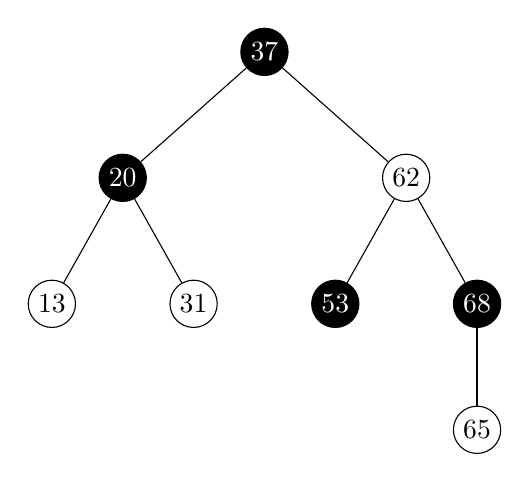
\begin{tikzpicture}[>={Stealth[length=2mm]}]
  \node[blacknode] (n0) at (2.70, 0.00) {37};
  \node[blacknode] (n1) at (0.90, -1.60) {20};
  \node[rednode] (n2) at (0.00, -3.20) {13};
  \node[rednode] (n3) at (1.80, -3.20) {31};
  \node[rednode] (n4) at (4.50, -1.60) {62};
  \node[blacknode] (n5) at (3.60, -3.20) {53};
  \node[blacknode] (n6) at (5.40, -3.20) {68};
  \node[rednode] (n7) at (5.40, -4.80) {65};
  \draw (n1) -- (n2);
  \draw (n1) -- (n3);
  \draw (n0) -- (n1);
  \draw (n4) -- (n5);
  \draw (n6) -- (n7);
  \draw (n4) -- (n6);
  \draw (n0) -- (n4);
\end{tikzpicture}
\end{center}

\end{document}
